\section{Experiments}

\subsection{Setups}
\noindent \textbf{Models and Benchmarks.} We evaluate our approach on several variants of two models: LLaDA-8B-Instruct \cite{llada}, LLaDA-1.5 \cite{llada1.5}, Dream-v0-Base-7B \cite{dream}, Dream-v0-Instruct-7B. Benchmarks include diverse datasets: GSM8K (5-shot) \cite{gsm8k}, MATH (4-shot) \cite{math}, HumanEval (0-shot) \cite{humaneval}, and MBPP (3-shot) \cite{mbpp}, covering a range of reasoning and code generation tasks. 
% We report the number of function evaluations (NFE) and tokens per second (TPS) to reflect speed, along with task accuracy. 
We report tokens per second (TPS), relative speedup ratio (Speedup) and number of function evaluations (NFE) to reflect efficiency, along with task accuracy (Acc.).

\noindent \textbf{Baselines.} We compare \dawn{} against four baselines: the Original sampling method (Top-1 Sampling), which unmasks the top-1 confidence position at each iteration; the Confidence-Aware Parallel proposed by Fast-dLLM \cite{fastdllm}, selecting positions whose confidence exceeds a predefined threshold; KLASS \cite{klass}, using both confidence and KL divergence to select positions; and LocalLeap \cite{localleap}, identifying anchors and performing localized relaxed parallel decoding. 

\noindent \textbf{Hardware and Implementation Details.} Our experiments are conducted on a NVIDIA H100 80G GPU. We set the generation length to 256 and the block length to 32 for all methods except KLASS, which uses its best-performing block length. All baselines are evaluated under their default hyperparameter settings. For \dawn{}, we average the attention maps from the last 4 layers. $\tau_{high}$ is set to 0.9 according to Fast-dLLM. Confidence thresholds are set from 0.7 to 0.85. Full configurations and the justifications can be found in Appendix~\ref{apdx: expdetails}. All evaluations are conducted using the standardized lm-eval \cite{lm-eval} library. 

\subsection{Main Results}

\begin{table*}[t!]
  \centering
  \small
  \caption{\textbf{Performance comparison between \dawn{} and baselines across 4 datasets and 4 models}. We report Accuracy, TPS, and Speedup to assess their efficiency and generation quality.}
  \label{tab:main_results}
  \resizebox{\textwidth}{!}{
    \begin{tabular}{c*{4}{ccc}}
      \toprule
        & \multicolumn{3}{c}{GSM8K}
        & \multicolumn{3}{c}{MATH}
        & \multicolumn{3}{c}{HumanEval}
        & \multicolumn{3}{c}{MBPP}\\
      \cmidrule(lr){2-4} \cmidrule(lr){5-7} \cmidrule(lr){8-10} \cmidrule(lr){11-13} 
      Method
        & Acc.$\uparrow$ & TPS$\uparrow$ & Speedup$\uparrow$
        & Acc.$\uparrow$ & TPS$\uparrow$ & Speedup$\uparrow$
        & Acc.$\uparrow$ & TPS$\uparrow$ & Speedup$\uparrow$
        & Acc.$\uparrow$ & TPS$\uparrow$ & Speedup$\uparrow$\\
      \midrule
      \multicolumn{13}{c}{LLaDA-8B-Instruct}\\
      \midrule
      Original & 77.94 & 10.32 & 1.00$\times$ & 33.20 & 14.10 & 1.00$\times$ & 40.24 & 26.46 & 1.00$\times$ & 29.60 & 9.46 & 1.00$\times$\\
      Confidence & 78.39 & 33.44 & 3.24$\times$ & 32.98 & 36.88 & 2.62$\times$ & 40.85 & 86.73 & 3.28$\times$ & 30.00 & 34.81 & 3.68$\times$\\
      KLASS & 76.12 & 23.23 & 2.25$\times$ & 32.32 & 25.27 & 1.79$\times$ & 36.59 & 56.91 & 2.15$\times$ & 27.00 & 22.62 & 2.39$\times$\\
      LocalLeap & 77.33 & 44.19 & 4.28$\times$ & 32.42 & 47.12 & 3.34$\times$ & 39.63 & \textbf{109.80} & \textbf{4.15$\times$} & 30.80 & 44.13 & 4.66$\times$\\
      \dawn{} & 77.94 & \textbf{44.72} & \textbf{4.33$\times$} & 32.36 & \textbf{48.16} & \textbf{3.42$\times$} & 40.24 & 108.99 & 4.12$\times$ & 30.80 & \textbf{45.17} & \textbf{4.77$\times$} \\
      \midrule
      \multicolumn{13}{c}{LLaDA-1.5}\\
      \midrule
      Original & 81.12 & 9.65 & 1.00$\times$ & 33.36 & 12.75 & 1.00$\times$ & 43.90 & 9.26 & 1.00$\times$ & 38.80 & 3.45 & 1.00$\times$\\
      Confidence & 80.74 & 32.49 & 3.37$\times$ & 33.38 & 32.87 & 2.58$\times$ & 42.68 & 23.39 & 2.53$\times$ & 38.80 & 20.40 & 5.91$\times$\\
      KLASS & 77.63 & 22.63 & 2.35$\times$ & 31.80 & 23.29 & 1.83$\times$ & 39.63 & 16.49 & 1.78$\times$ & 30.00 & 13.25 & 3.84$\times$\\
      LocalLeap & 80.14 & 42.60 & 4.41$\times$ & 32.44 & 42.36 & 3.32$\times$ & 42.07 & \textbf{30.21} & \textbf{3.26$\times$} & 39.20 & 27.00 & 7.83$\times$\\
      \dawn{} & 80.82 & \textbf{43.24} & \textbf{4.48$\times$} & 31.80 & \textbf{42.84} & \textbf{3.36$\times$} & 42.07 & 29.53 & 3.19$\times$ & 37.60 & \textbf{27.80} & \textbf{8.06$\times$} \\
      \midrule
      \multicolumn{13}{c}{Dream-v0-Base-7B}\\
      \midrule
      Original & 76.42 & 14.37 & 1.00$\times$ & 34.70 & 18.16 & 1.00$\times$ & 38.41 & 20.90 & 1.00$\times$ & 53.40 & 11.85 & 1.00$\times$\\
      Confidence & 73.84 & 23.41 & 1.63$\times$ & 34.38 & 44.66 & 2.46$\times$ & 39.63 & 61.54 & 2.94$\times$ & 53.80 & 50.37 & 4.25$\times$\\
      KLASS & 72.00 & 12.58 & 0.88$\times$ & 32.80 & 23.16 & 1.27$\times$ & 42.68 & 31.32 & 1.50$\times$ & 55.80 & 19.46 & 1.64$\times$\\
      LocalLeap & 72.55 & 25.40 & 1.77$\times$ & 34.48 & 51.32 & 2.83$\times$ & 36.59 & 68.28 & 3.27$\times$ & 53.60 & 59.38 & 5.01$\times$\\
      \dawn{} & 73.54 & \textbf{25.88} & \textbf{1.80$\times$} & 34.00 & \textbf{51.45} & \textbf{2.83$\times$} & 39.63 & \textbf{68.96} & \textbf{3.29$\times$} & 53.20 & \textbf{64.55} & \textbf{5.45$\times$} \\
      \midrule 
      \multicolumn{13}{c}{Dream-v0-Instruct-7B}\\
      \midrule
      Original & 76.35 & 7.30 & 1.00$\times$ & 37.80 & 17.73 & 1.00$\times$ & 53.66 & 22.66 & 1.00$\times$ & 54.20 & 8.37 & 1.00$\times$\\
      Confidence & 75.20 & 28.81 & 3.95$\times$ & 38.24 & 37.92 & 2.14$\times$ & 57.32 & 52.11 & 2.30$\times$ & 55.60 & 39.09 & 4.67$\times$\\
      KLASS & 71.72 & 12.93 & 1.77$\times$ & 34.66 & 18.74 & 1.06$\times$ & 54.88 & 26.71 & 1.18$\times$ & 56.80 & 18.53 & 2.21$\times$\\
      LocalLeap & 73.24 & 32.94 & 4.51$\times$ & 38.10 & 43.66 & 2.46$\times$ & 54.27 & 59.28 & 2.62$\times$ & 55.00 & 42.71 & 5.10$\times$\\
      \dawn{} & 73.16 & \textbf{32.99} & \textbf{4.52$\times$} & 38.22 & \textbf{44.18} & \textbf{2.49$\times$} & 54.88 & \textbf{60.23} & \textbf{2.66$\times$} & 55.80 & \textbf{44.03} & \textbf{5.26$\times$} \\
      \bottomrule
    \end{tabular}
  }
\end{table*}

% \begin{table*}[t!]
%   \centering
%   \small
%   \caption{\textbf{Main results}, which contain the performance comparison between \dawn{} and the
% baselines across 4 datasets and 4 models. We report Accuracy, TPS, and NFE in each cell to assess their efficiency and quality. The generation length is 256, block size is 32.}\label{tab:main_results}
%   \resizebox{\textwidth}{!}{
%     \begin{tabular}{c*{4}{ccc}}
%       \toprule
%         & \multicolumn{3}{c}{GSM8K}
%         & \multicolumn{3}{c}{MATH}
%         & \multicolumn{3}{c}{HumanEval}
%         & \multicolumn{3}{c}{MBPP}\\
%       \cmidrule(lr){2-4} \cmidrule(lr){5-7} \cmidrule(lr){8-10} \cmidrule(lr){11-13} 
%       Method
%         & Acc.$\uparrow$ & TPS$\uparrow$ & NFE$\downarrow$
%         & Acc.$\uparrow$ & TPS$\uparrow$ & NFE$\downarrow$
%         & Acc.$\uparrow$ & TPS$\uparrow$ & NFE$\downarrow$
%         & Acc.$\uparrow$ & TPS$\uparrow$ & NFE$\downarrow$\\
%       \midrule
%       \multicolumn{13}{c}{LLaDA-8B-Instruct}\\
%       \midrule
%       Original & 77.94 & 10.32 & 256.00 & XX & XX & 256.00 & 40.24 & 26.46 & 256.00 & 29.60 & 9.46 & 256.00\\
%       Confidence & 78.39 & 33.44 & 78.60 & 32.98 & 36.88 & 96.99 & 40.85 & 86.73 & 77.38 & 30.00 & 34.81 & 69.14\\
%       KLASS & XX & XX & XX & XX & XX & XX & XX & XX & XX & XX & XX & XX\\
%       LocalLeap & 77.33 & 44.19 & 58.99 & 32.42 & 47.12 & 75.60 & 39.63 & 109.80 & 61.02 & 30.80 & 44.13 & 54.26\\
%       \dawn{} & 77.94 & 44.72 & 55.76 & 32.36 & 48.16 & 72.40 & 40.24 & 108.99 & 61.63 & 30.80 & 45.17 & 50.23\\
%       \midrule
%       \multicolumn{13}{c}{LLaDA-1.5}\\
%       \midrule
%       Original & 81.12 & 9.65 & 256.00 & XX & XX & XX & XX & XX & XX & XX & XX & XX\\
%       Confidence & 80.74 & 32.49 & 75.34 & 33.38 & 32.87 & 95.68 & 42.68 & 23.39 & 101.07 & 38.80 & 20.40 & 42.18\\
%       KLASS & XX & XX & XX & XX & XX & XX & XX & XX & XX & XX & XX & XX\\
%       LocalLeap & 80.14 & 42.60 & 57.54 & 32.44 & 42.36 & 75.70 & 42.07 & 30.21 & 76.37 & 39.20 & 27.00 & 32.04\\
%       \dawn{} & 80.82 & 43.24 & 54.36 & 31.80 & 42.84 & 72.88 & 42.07 & 29.53 & 78.18 & 37.60 & 27.80 & 28.58\\
%       \midrule
%       \multicolumn{13}{c}{Dream-v0-Base-7B}\\
%       \midrule
%       Original & 76.42 & 14.37 & 256.00 & XX & XX & 256.00 & 38.41 & 20.90 & 256.00 & 53.40 & 11.85 & 256.00\\
%       Confidence & 73.84 & 23.41 & 152.43 & XX & XX & XX & 39.63 & 61.54 & 133.29 & 53.80 & 50.37 & 89.90\\
%       KLASS & XX & XX & XX & XX & XX & XX & XX & XX & XX & XX & XX & XX\\
%       LocalLeap & 72.55 & 25.40 & 140.16 & 34.48 & 51.32 & 87.94 & 36.59 & 68.28 & 119.24 & 53.60 & 59.38 & 76.22\\
%       \dawn{} & 73.54 & 25.88 & 135.19 & 34.00 & 51.45 & 86.34 & 39.63 & 68.96 & 119.91 & 53.20 & 64.55 & 68.97\\
%       \midrule 
%       \multicolumn{13}{c}{Dream-v0-Instruct-7B}\\
%       \midrule
%       Original & 76.35 & 7.30 & 256.00 & XX & XX & 256.00 & 53.66 & 22.66 & 256.00 & 54.20 & 8.37 & 256.00\\
%       Confidence & 75.20 & 28.81 & 62.59 & XX & XX & XX & 57.32 & 52.11 & 93.63 & 55.60 & 39.09 & 62.79\\
%       KLASS & XX & XX & XX & XX & XX & XX & XX & XX & XX & XX & XX & XX\\
%       LocalLeap & 73.24 & 32.94 & 54.17 & 38.10 & 43.66 & 97.81 & 54.27 & 59.28 & 79.11 & 55.00 & 42.71 & 45.11\\
%       \dawn{} & 73.16 & 32.99 & 51.92 & 38.22 & 44.18 & 94.52 & 54.88 & 60.23 & 76.71 & 55.80 & 44.03 & 42.90\\
%       \bottomrule
%     \end{tabular}
%   }
% \end{table*}

Table~\ref{tab:main_results} reports the accuracy and efficiency of each method across different models on four benchmarks.

Overall, \dawn{} achieves a substantial improvement in inference speed while maintaining accuracy comparable to or even slightly higher than the original method. \dawn{} achieves substantially higher throughput than prior decoding baselines, with up to \textbf{8.06$\times$} speedup on MBPP using the LLaDA-1.5 model. Moreover, these gains do not come at the cost of quality. On LLaDA-8B-Instruct, \dawn{} achieves 77.94 accuracy on GSM8K, matching the original method, and attains 30.80 on MBPP, slightly higher than the original 29.60. In other settings, \dawn{} incurs only negligible quality loss, indicating a more favorable quality--speed trade-off. 

Compared with confidence-aware parallel and KLASS, \dawn{} significantly improves throughput while achieving nearly identical accuracy. Compared with LocalLeap, \dawn{} shows clear advantages in both quality and speed: across most benchmarks, it improves throughput by approximately 0.05 – 5.17 tokens per second while enhancing accuracy by up to 3.04\%. It unlocks additional safe parallelism by explicitly accounting for positional dependencies during refinement, enabling more efficient decoding. 

\subsection{Ablation Study}

% \begin{table}[t!]
%   \centering
%   \small
%   \caption{\textbf{Ablation study}, which verifies the effectiveness of modules of \dawn{} across 2 datasets and 2 models. We report Accuracy and TPS to assess their efficiency and quality. The settings are the same as in the main experiments.}\label{tab:ablation}
%   \resizebox{\columnwidth}{!}{
%     \begin{tabular}{c*{2}{ccc}}
%       \toprule
%         & \multicolumn{2}{c}{GSM8K}
%         & \multicolumn{2}{c}{HumanEval}\\
%       \cmidrule(lr){2-3} \cmidrule(lr){4-5}
%       Method
%         & Acc.$\uparrow$ & TPS$\uparrow$ 
%         & Acc.$\uparrow$ & TPS$\uparrow$\\
%       \midrule
%       \multicolumn{5}{c}{LLaDA-8B-Instruct}\\
%       \midrule
%       Original & XX & XX & XX & XX \\
%       % \dawn{} w/o DGC & XX & XX & XX & XX \\
%       \dawn{} w/o AGD & XX & XX & XX & XX \\
%       \dawn{} w/o CBS & XX & XX & XX & XX \\
%       \dawn{} & XX & XX & XX & XX \\
%       \midrule 
%       \multicolumn{5}{c}{Dream-v0-Instruct-7B}\\
%       \midrule
%       Original & XX & XX & XX & XX \\
%       % \dawn{} w/o DGC & XX & XX & XX & XX \\
%       \dawn{} w/o AGD & XX & XX & XX & XX \\
%       \dawn{} w/o CBS & XX & XX & XX & XX \\
%       \dawn{} & XX & XX & XX & XX \\
%       \bottomrule
%     \end{tabular}
%   }
% \end{table}

We conduct extensive ablation studies to assess the contributions of key components in \dawn{}. We further examine the sensitivity of \dawn{} to the generation length and the lower confidence threshold $\tau_{low}$ to understand how these factors affect its effectiveness. Discussions of other hyperparameter choices are provided in Appendix~\ref{apdx: expdetails}. All other experiment settings follow the main experiment.

\begin{table}[t!]
  \centering
  \small
  \caption{\textbf{Ablation study on the effectiveness of key modules in \dawn{} across 2 datasets and 2 models}. We report Accuracy, TPS, and NFE to assess their quality and speed. The settings are the same as in the main experiments.}\label{tab:ablation}
  \resizebox{\columnwidth}{!}{
    \begin{tabular}{c*{2}{ccc}}
      \toprule
        & \multicolumn{3}{c}{GSM8K}
        & \multicolumn{3}{c}{HumanEval}\\
      \cmidrule(lr){2-4} \cmidrule(lr){5-7}
      Method
        & Acc.$\uparrow$ & TPS$\uparrow$ & NFE$\downarrow$ 
        & Acc.$\uparrow$ & TPS$\uparrow$ & NFE$\downarrow$  \\
      \midrule
      \multicolumn{7}{c}{LLaDA-8B-Instruct}\\
      \midrule
      \dawn{} & 77.94 & \textbf{44.72} & \textbf{55.76} & 40.24 & \textbf{109.0} & \textbf{61.63} \\
      % \dawn{} w/o DGC & XX & XX & XX & XX & XX & XX \\
      - AGD & 76.80 & 22.31 & 112.9 & \textbf{41.46} & 51.51 & 131.0 \\
      - CBS & \textbf{78.47} & 33.83 & 74.69 & 41.46 & 92.52 & 72.93 \\
      Original & 77.94 & 10.32 & 256 & 40.24 & 26.46 & 256 \\
      \midrule 
      \multicolumn{7}{c}{Dream-v0-Instruct-7B}\\
      \midrule
      \dawn{} & 73.16 & \textbf{32.99} & \textbf{51.92} & 54.88 & \textbf{60.23} & \textbf{77.12} \\
      % \dawn{} w/o DGC & XX & XX & XX & XX & XX & XX \\
      - AGD & 73.31 & 29.33 & 58.13 & 54.88 & 54.79 & 83.34 \\
      - CBS & 75.28 & 27.63 & 62.19 & \textbf{57.31} & 51.97 & 93.01 \\
      Original & \textbf{76.35} & 7.30 & 256 & 53.66 & 22.66 & 256 \\
      \bottomrule
    \end{tabular}
  }
\end{table}

\noindent \textbf{Effectiveness of key components.} Since \textit{Dependency Graph Construction} serves as the foundation for the other two modules, we focus on validating the effectiveness of components for selecting parallel update positions. Table~\ref{tab:ablation} summarizes ablations of \dawn{} on two representative dLLMs and benchmarks. Overall, the full solution consistently improves efficiency while maintaining comparable accuracy. In particular, removing \textit{Anchor-Guided Decoding} (AGD) causes a substantial efficiency drop across both models and tasks. On LLaDA-8B-Instruct, TPS decreases from $44.72$ to $22.31$ on GSM8K, indicating that AGD is a primary contributor to the speedup by expanding the set of positions that can be safely unmasked under reliable anchor context. On Dream-v0-Instruct-7B, removing \textit{Conflict-Based Scheduling} (CBS) yields higher accuracy but lower efficiency, suggesting that CBS mainly unlocks additional parallelism by avoiding inconsistent joint updates among strongly coupled positions, trading a small amount of accuracy for further acceleration.

\begin{figure}[t!]
    \centering
    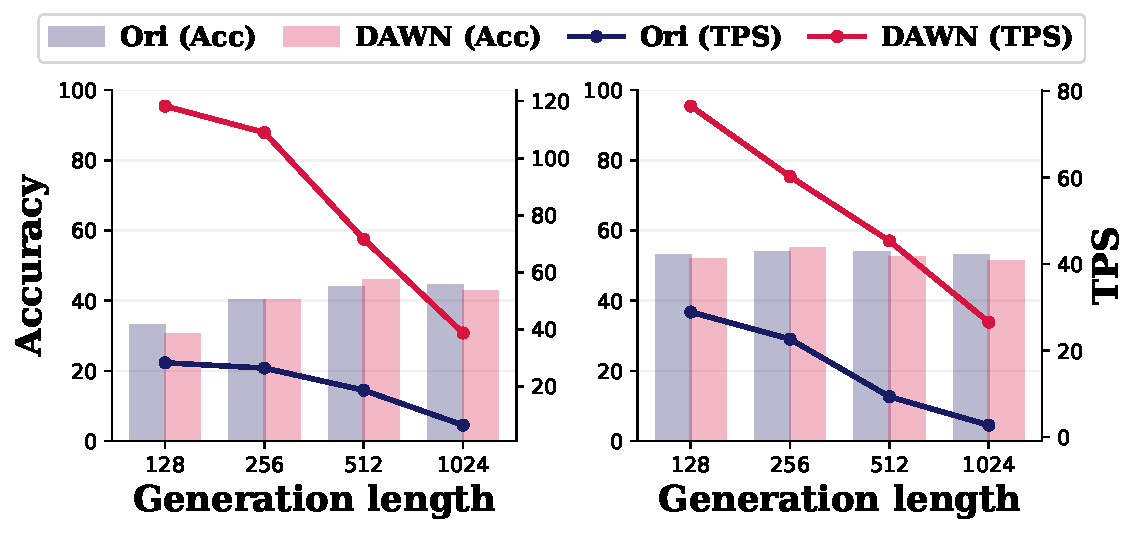
\includegraphics[width=\columnwidth]{fig/len_ablation.pdf}
    \caption{\textbf{Effectiveness of \dawn{} and the original sampler on HumanEval under different generation lengths ($L\in\{128,256,512,1024\}$)}. Bars report accuracy (left y-axis) and solid lines report TPS (right y-axis). Left and right figures correspond to LLaDA-8B-Instruct and Dream-v0-Instruct-7B.}
    \label{fig:len_abl}
\end{figure}

\noindent \textbf{Impact of generation length.} Figure~\ref{fig:len_abl} reports the accuracy and throughput of \dawn{} and the original baseline with different generation lengths $L$. Across both LLaDA and Dream models, \dawn{} consistently improves throughput over the original sampler while maintaining comparable accuracy. As $L$ increases, throughput decreases for both methods due to higher denoising costs, yet \dawn{} continues to boost the efficiency. Overall, it preserves a more favorable quality-speed trade-off across a wide range of lengths.

\begin{figure}[t!]
    \centering
    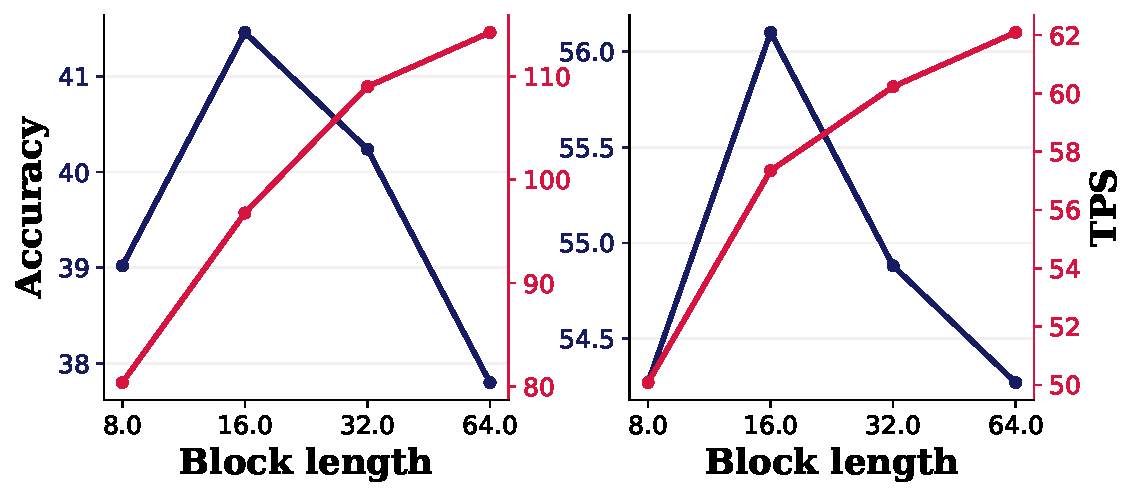
\includegraphics[width=\columnwidth]{fig/ablation_blocklen_equal_spacing.pdf}
    \caption{\textbf{Effectiveness of \dawn{} on HumanEval under different block lengths ($L\in\{8,16,32,64\}$)}. We report accuracy (blue, left y-axis) and TPS (red, right y-axis). Left and right figures correspond to LLaDA-8B-Instruct and Dream-v0-Instruct-7B.}
    \label{fig:blen_abl}
\end{figure}

\noindent \textbf{Impact of block length.} Figure~\ref{fig:blen_abl} reports the accuracy and throughput of \dawn{} with different block lengths. As the block length increases, throughput increases for both methods as higher parallelism, but accuracy first increases and then decreases. Overall, it preserves a  robust quality-speed trade-off across a wide range of lengths.

\begin{figure}[t!]
    \centering
    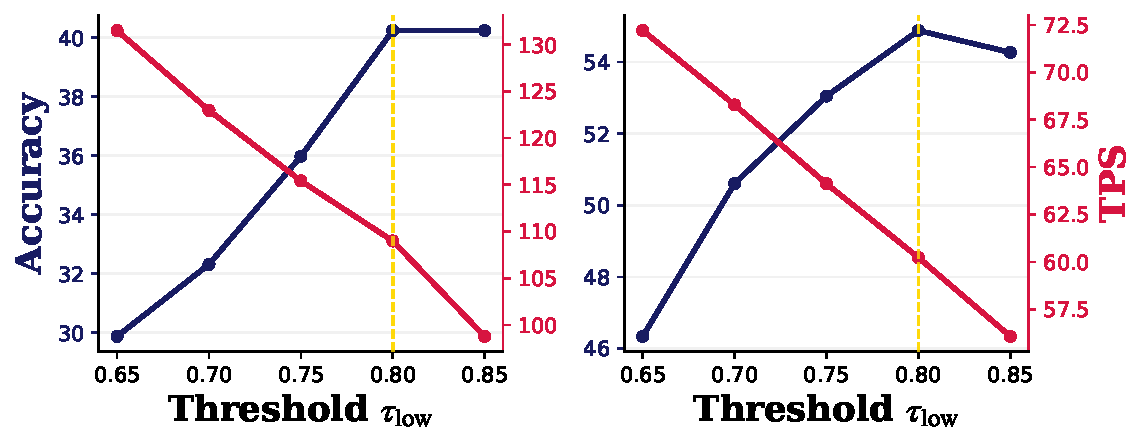
\includegraphics[width=\columnwidth]{fig/ablation_conf.pdf}
    \caption{\textbf{We vary the lower threshold $\tau_{low}$ and report accuracy (blue, left y-axis) and throughput TPS (red, right y-axis) on HumanEval}. The left and right figures correspond to LLaDA-8B-Instruct and Dream-v0-Instruct-7B. The dashed line (yellow) marks the default setting $\tau_{low}=0.80$.}
    \label{fig:conf_abl}
\end{figure}

\noindent \textbf{Impact of lower threshold.} Figure~\ref{fig:conf_abl} reports the evaluation under different values of lower threshold $\tau_{low}$. We observe a clear quality-speed trade-off on both models. Reducing $\tau_{low}$ increases TPS by admitting more parallel updates, but can hurt accuracy due to less reliable low-confidence commitments. 
% Conversely, increasing $\tau_{low}$ improves accuracy while decreasing throughput. 
The default $\tau_{low}=0.80$ (dashed line) maintains a high generation quality and improved efficiency.

